\documentclass{article}

%\usepackage[version=3]{mhchem} % Package for chemical equation typesetting
\usepackage{siunitx} % Provides the \SI{}{} and \si{} command for typesetting SI units
\usepackage{graphicx} % Required for the inclusion of images
\usepackage{natbib} % Required to change bibliography style to APA
\usepackage{amsmath} % Required for some math elements 

\usepackage{fancyhdr}


\usepackage[margin = 1in]{geometry} %set the margin

%----------------------------------------------------------------------------------------
%	DOCUMENT INFORMATION
%----------------------------------------------------------------------------------------
%

\begin{document}

\begin{figure}
\centering
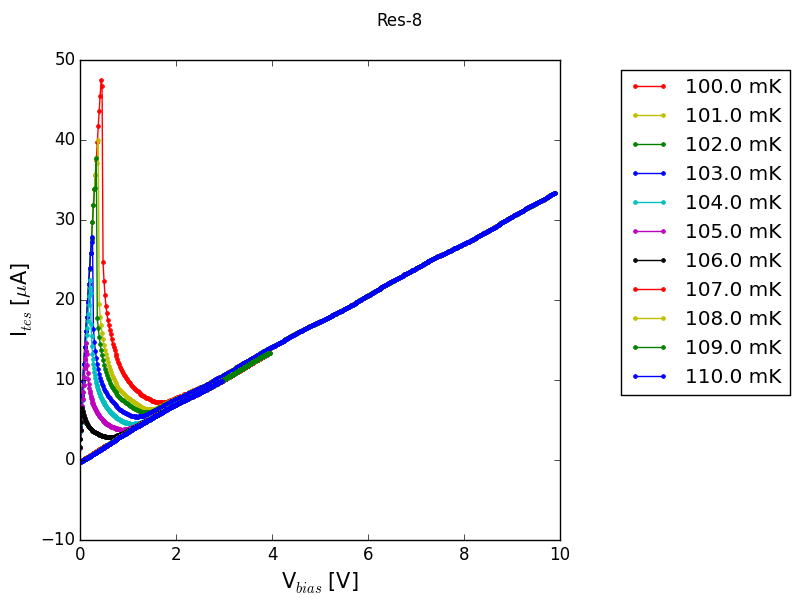
\includegraphics[width=.8\linewidth,keepaspectratio]{Res-8_1}
\end{figure}

\begin{figure}
\centering
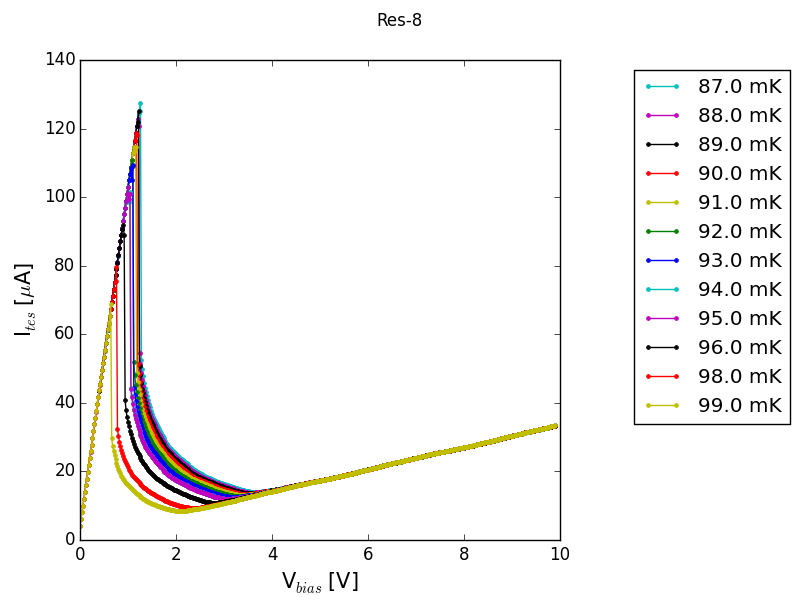
\includegraphics[width=.8\linewidth,keepaspectratio]{Res-8_2}
\caption{Res-8, 5.096 GHz, TES-6, SQUID-13}
\end{figure}

\begin{figure}
\centering
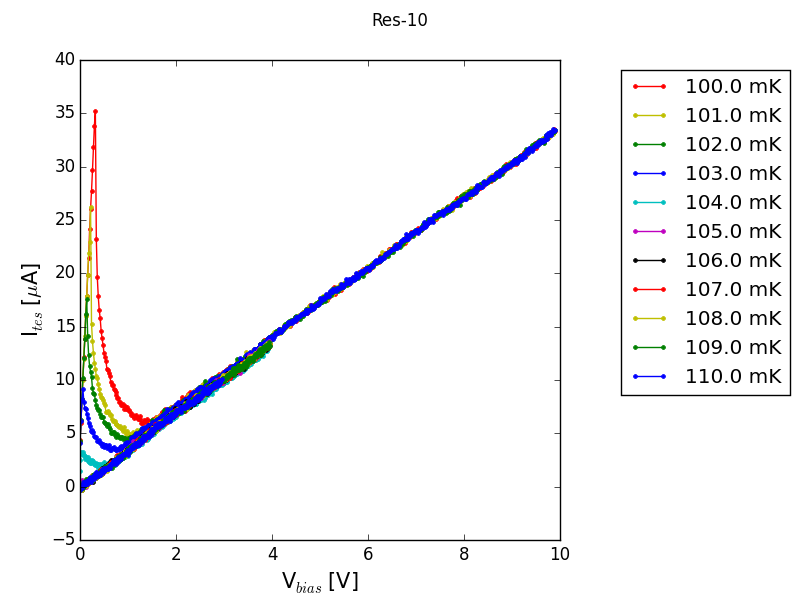
\includegraphics[width=.8\linewidth,keepaspectratio]{Res-10_1}
\end{figure}

\begin{figure}
\centering
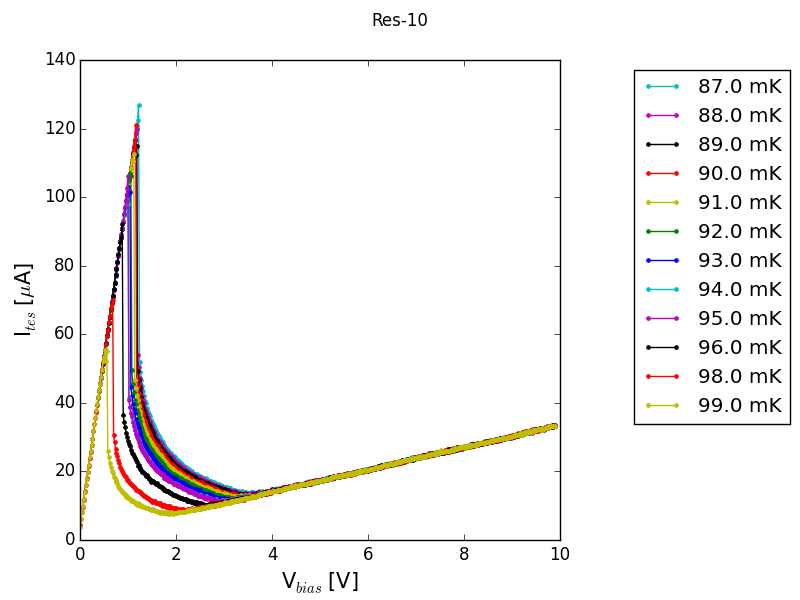
\includegraphics[width=.8\linewidth,keepaspectratio]{Res-10_2}
\caption{Res-10, 5.110 GHz, TES-10, SQUID-17}
\end{figure}


\begin{figure}
\centering
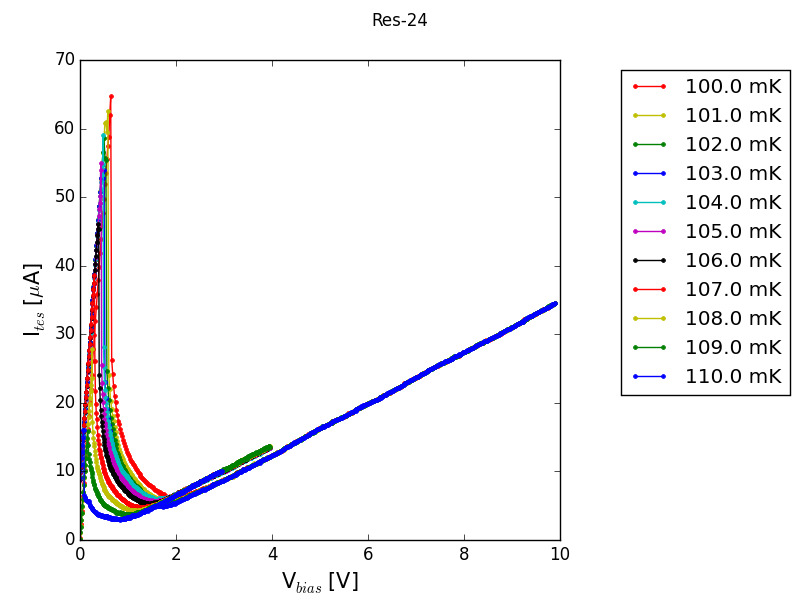
\includegraphics[width=.8\linewidth,keepaspectratio]{Res-24_1}
\end{figure}

\begin{figure}
\centering
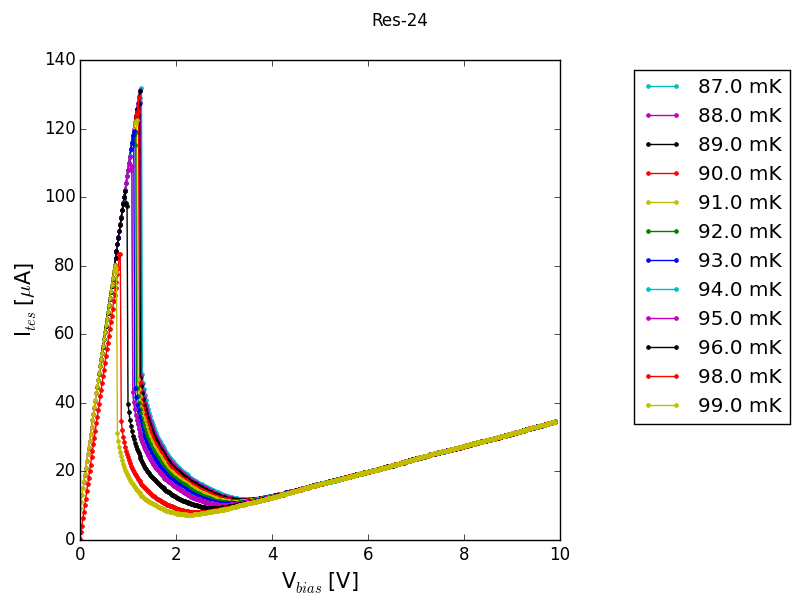
\includegraphics[width=.8\linewidth,keepaspectratio]{Res-24_2}
\caption{Res-24, 5.199 GHz, TES-5, SQUID-12}
\end{figure}

\end{document}